\documentclass{article}

\usepackage{graphicx}
\usepackage{tikz}
\usepackage{tikzsymbols}
\usetikzlibrary{calc,patterns,shapes.geometric}
\pagestyle{empty}
\usepackage[margin=0pt]{geometry}
\geometry{papersize={14in,12in}}

\def\centerarc[#1](#2)(#3:#4:#5){\draw[#1] ($(#2)+({#5*cos(#3)},{#5*sin(#3)})$) arc (#3:#4:#5);}

\begin{document}
	\begin{figure}
		\centering
		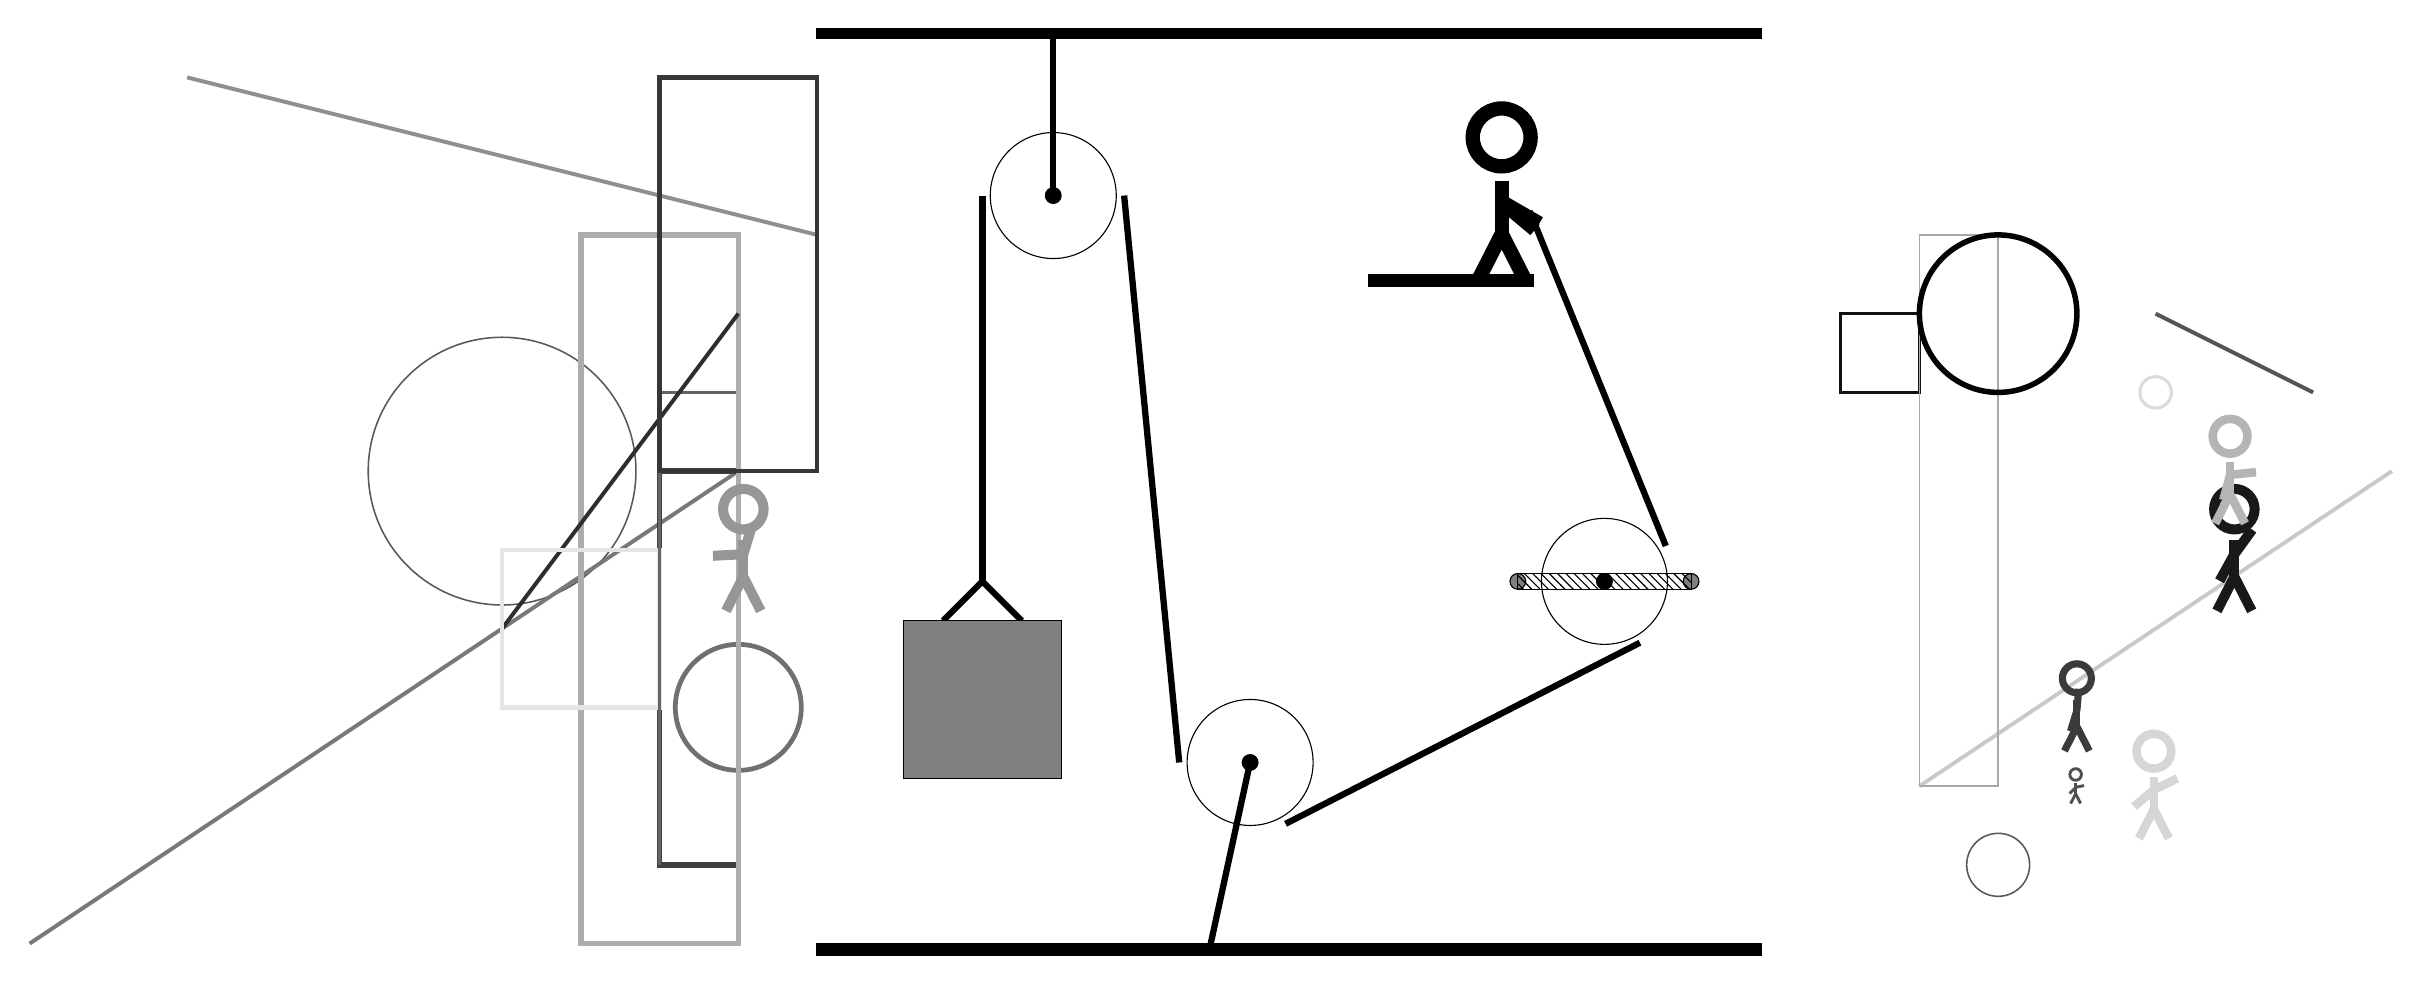
\begin{tikzpicture}
			%%%%% START %%%%%
			
			\draw[fill=black] (-2, 11.5) rectangle (10, 11.625);
			
			\draw [line width=0.4mm, color=black!14](15, 7) circle (0.2);
			
			\draw[line width=0.4mm, color=black!61] (-4, 7) rectangle (-3, 9);
			\draw[line width=0.4mm, color=black!44] (-2, 9) rectangle (-2, 9);
			\draw[line width=0.5mm, color=black!21](12, 2) -- (18, 6);
			
			\draw[line width=0.4mm, color=black!93] (12, 8) rectangle (11, 7);
			
			\draw[line width=0.2mm, color=black!34] (12, 2) rectangle (13, 9);
			\node[line width=0.3mm, color=black!69] at (14, 2) {\Strichmaxerl[2][46][12]};
			\draw [line width=0.6mm, color=black!56](-3, 3) circle (0.8);
			\node[line width=0.4mm, color=black!90] at (16, 5) {\Strichmaxerl[7][61][54]};
			\node[line width=0.7mm, color=black!16] at (15, 2) {\Strichmaxerl[6][40][26]};
			\draw [line width=0.2mm, color=black!65](-6, 6) circle (1.7);
			\draw[line width=0.5mm, color=black!53](-3, 6) -- (-12, 0);
			\draw[line width=0.7mm, color=black!75] (-3, 6) rectangle (-4, 1);
			
			\draw[line width=0.7mm, color=black!32] (-3, 9) rectangle (-5, 0);
			\draw [line width=0.7mm, color=black!99](13, 8) circle (1.0);
			\draw[line width=0.5mm, color=black!44](-2, 9) -- (-10, 11);
			\draw[line width=0.5mm, color=black!67](15, 8) -- (17, 7);
			\node[line width=0.6mm, color=black!29] at (16, 6) {\Strichmaxerl[6][75][6]};
			\draw[line width=0.5mm, color=black!82](-6, 4) -- (-3, 8);
			\node[line width=0.4mm, color=black!77] at (14, 3) {\Strichmaxerl[5][73][85]};
			\draw[line width=0.6mm, color=black!10] (-4, 5) rectangle (-6, 3);
			\draw[line width=0.3mm, color=black!60] (-4, 1) rectangle (-4, 9);
			\node[line width=0.3mm, color=black!41] at (-3, 5) {\Strichmaxerl[7][3][73]};
			\draw [line width=0.2mm, color=black!65](13, 1) circle (0.4);
			\draw[line width=0.6mm, color=black!79] (-2, 6) rectangle (-4, 11);
			
			
			\draw (1, 9.5) circle (0.8);
			\draw[fill=black] (1, 9.5) circle (0.1);
			\draw[line width=0.8mm] (1, 11.5) -- (1, 9.5);
			
			\draw (3.5, 2.3) circle (0.8);
			\draw[fill=black] (3.5, 2.3) circle (0.1);
			\draw[line width=0.8mm] (3.5, 2.3) -- (3.0, 0);
			
			\draw[fill=white](8, 4.6) circle (0.8);
			\draw[fill=black] (8, 4.6) circle (0.1);
			\draw[fill=black!50] (9.1, 4.6) circle (0.1);
			\draw[fill=black!50] (6.9, 4.6) circle (0.1);
			\draw[pattern=north west lines, pattern color=black] (6.9, 4.7) rectangle (9.1, 4.5);
			
			\draw[line width=0.8mm](-0.4, 4.1) --  (0.1, 4.6) -- (0.6, 4.1);
			\draw[fill=black!50] (-0.9, 4.1) rectangle (1.1, 2.1);
			
			\draw[line width=0.8mm](0.1, 9.5) -- (0.1, 4.6);
			\centerarc[line width=0.8mm](1, 9.5)(180:0:0.9)
			\draw[line width=0.8mm](1.9, 9.5) -- (2.6, 2.3);
			\centerarc[line width=0.8mm](3.5, 2.3)(180:300:0.9);
			\draw[line width=0.8mm](3.95, 1.5206) -- (8.45, 3.8206);
			\centerarc[line width=0.8mm](8, 4.6)(300:390:0.9);
			\draw[line width=0.8mm](8.7794, 5.05) -- (7.05, 9.3);
			
			\node at (6.75, 9.5) {\Strichmaxerl[10][-220][-30]};
			\draw[fill=black] (5, 8.5) rectangle (7.1, 8.35);
			
			\draw[fill=black] (-2, 0) rectangle (10, -0.15);
			
			%%%%% END %%%%%
		\end{tikzpicture}
	\end{figure}	
\end{document}